\chapter{Расчёт параметров}

\section{Расчёт относительного уменьшения возбуждения на краю антенны}

Для обеспечения требуемого УБЛ используем распределение со спадающей к краям амплитудой вида косинус на пьедестале.
$t\approx-(13+13\Delta+22\Delta^2)$
Решив квадратное уравнение получим $\Delta=0.3$.
\section{Расчёт межелементного расстояния}
Для углов $\theta_\text{ск}\leq45^\circ$ можно применять <<мягкую>>  формулу:

$\displaystyle d\leq\frac{\lambda}{sin\theta_\text{Д}+sin\theta_\text{ск}}$, где $\theta_\text{Д}$ -- направление дифракционного максимума, которое мы найдём, воспользовавшись формулой для аппроксимации ДН элемента: \par\noindent
\begin{fleqn}
\[f(\theta)=cos^a(\theta)                                     \]
\[cos^{2\alpha}\theta^{\circ}_{\text{ск}}=1/2                 \]
\[\alpha=0.5\cdot\frac{log0.5}{log(cos(18^\circ))}=6.91       \]
\[cos^{2\alpha}\theta^{\circ}_{\text{Д}}=t=0.013              \]
\[\theta_\text{Д}=arccos(\sqrt[2\alpha]{t_\text{ед}})=43.24   \]
\end{fleqn}


Отсюда $d=5.03 \text{ см}$


\section{Расчёт количества элементов}

Из формулы для вычисления количества элементов по заданным $\Delta\theta_{0.5}$ и $\Delta$ найдём $N_1$ и $N_2$ -- число элементов на каждой стороне антенны.

\[N_1=\frac{(1+0.636\cdot\Delta^2)\cdot51^\circ\cdot\lambda}{\theta_{0.5x}\cdot d}=18\]

\[N_2=\frac{(1+0.636\cdot\Delta^2)\cdot51^\circ\cdot\lambda}{\theta_{0.5y}\cdot d}=14\] 

Линейный размер решётки равен $N_i\cdot d$, отсюда длина и ширина решетки 

$L=90.5 cm W=70.4 cm$

Общее число элементов $N=N_1\cdot N_2=252$

\section{Выбор схемы разводки и расчёт энергетического потенциала АФАР}

\subsection{Одноэтажная схема}
Рассмотрим одноэтажную схему разводки ( Рис. \ref{fig:1lev_rec_struct} ). Используем сумматор на 256. Неиспользуемые входы сумматора включим на согласованную нагрузку.
\begin{figure}[H]
	\centering
		
\includegraphics[width=0.7\textwidth]{1lev_rec_struct.pdf}
	\caption{Одноэтажная схема разводки}
	\label{fig:1lev_rec_struct}
\end{figure}

\begin{figure}[H]
	\centering
	\includegraphics[width=0.7\textwidth]{1lev_rec_channel.pdf}
	\caption{Схема прохождения сигнала по одному каналу}
	\label{fig:1lev_rec_channel}
\end{figure}

Условимся, что 
\begin{figure}[!h]
	\begin{tabularx}{1.5\textwidth}{>{\raggedright\arraybackslash}X >{\raggedright\arraybackslash}X}
		Погонные потери в соединительных кабелях (до МШУ) 	\dotfill & 1 дБ/м\\
		Потери на ФВ										\dotfill & 3 дБ\\
		Омические потери в одном сумматоре $L_{1\Sigma}$	\dotfill & 0.5 дБ\\
		Потери в соединительных кабелях 					\dotfill & 1 дБ\\
		Потери в соединительном кабеле между АФАР и ПРМ		\dotfill & 0.5 дБ
	\end{tabularx}
\end{figure}

Найдём потери в кабеле как $L_\text{каб}=l_\text{каб}\cdot\sqrt{L^2+W^2}/2=0.6 \text{ дБ}$

Возьмём потери в кабеле и фильтре МШУ $L_1=0.8\text{ дБ}=1.2$

$L_2=L_\text{ФВ}+L_\text{фид}+L_{1\Sigma}\cdot N_\text{э}=1+3+0.5\cdot8=8\text{ дБ}=6.3$

$L_3=0.5 \text{ дБ}=1.1$

$L_\Sigma=L_1+L_2+L_3=8.77 \text{ дБ}=7.5$

Рассчитаем $K_{\text{ш}_\Sigma}$

\begin{multline*} \displaystyle K_{\text{ш}_\Sigma}=K_\text{ш}L_1+\frac{(L_2-1)L_1}{K_p}+\frac{(K_\text{ш}-1)L_1L_2}{K_p}+\frac{(L_3-1)L_1L_2}{K^2_p}+\frac{L_1L_2L_3}{K^2_p}=\\=2.5+0.2+0.26+0.0009+0.0085=2.97 \end{multline*}

Отношение остальных слагаемых к первому около 18.8%

Проверим $\displaystyle \frac{L_\Sigma}{K_p}\leq 0.1\div0.5$

 $\displaystyle \frac{L_\Sigma}{K_p}=7.5/32=0.24$
 
 \subsection{Двухэтажная схема}
 Целесообразно применить активную разводку с двухэтажной схемой ( Рис. \ref{fig:2lev_rec_struct} ). Исходя из соображений баланса экономических затрат и коэффициента шума разбиваем решетку на 32 подрешетки по 8 элементов.
 
 \begin{figure}[H]
 	\centering
 	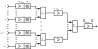
\includegraphics[width=0.9\textwidth]{2lev_rec_struct.pdf}
 	\caption{Двухэтажная схема разводки}
 	\label{fig:2lev_rec_struct}
 \end{figure}

\begin{figure}[H]
	\centering
	
\includegraphics[width=0.8\textwidth]{2lev_rec_channel.pdf}
	\caption{Схема прохождения сигнала по одному каналу}
	\label{fig:2lev_rec_channel}
\end{figure}

На Рис. \ref{fig:2lev_rec_channel} 

$L_1$ -- потери в соединительном кабеле между излучателем и МШУ, а так же потери во входном фильтре. $L_1=0.8\text{ дБ}=1.2$

$L_2$ -- потери в ФВ, первых сумматорах и соединительных кабелях.

$L_2=L_\text{ФВ}+L_\text{фид}+L_{1\Sigma}\cdot N_\text{э}=1+3+0.5\cdot3=5.5\text{ дБ}=3.6$

$L_3$ -- потери в остальных сумматорах и соединительных кабелях.

$L_3=L_\text{фид}+L_{1\Sigma}\cdot N_\text{э2}=1+0.5\cdot5=3.5 \text{ дБ}=2.2$

$L_4$ -- потери в соединительном кабеле между МШУ и ПРМ. $L_4=0.5 \text{ дБ}=1.1$

Для такой схемы коэффициент шума рассчитывается по следующей формуле:

\begin{multline*} \displaystyle K_{\text{ш}_\Sigma}=K_\text{ш}L_1+\frac{(L_2-1)L_1}{K_p}+\frac{(K_\text{ш}-1)L_1L_2}{K_p}+\frac{(L_3-1)L_1L_2}{K^2_p}+\frac{(K_\text{ш}-1)L_1L_2L_3}{K^2_p}+\\+\frac{(L_4-1)L_1L_2L_3}{K^2_p}+\frac{L_1L_2L_3L_4}{K^3_p} = 2.4966 + 0.0963 + 0.1460 + 0.0053 + 0.0103 = 2.75\end{multline*}

Отношение остальных слагаемых к первому около 10.3%

Проверим $\displaystyle \frac{L_\Sigma}{K_p}\leq 0.1\div0.5$

$\displaystyle \frac{L_\Sigma}{K_p}=4.7/32=0.12$

Необходимость перехода к 3этажной схеме отсутствует.

\subsection{Расчёт энергетического потенциала АФАР}

$\displaystyle \text{П}_\text{ПРМ}=\frac{S_\text{эфф}}{T_\text{эфф}}$


$\displaystyle S_\text{эфф}=A \cdot S_1 \cdot \sigma = A \cdot L \cdot W \cdot \sigma = 0.5\cdot90.5\cdot70.4\cdot0.7 = 2232$

$T_\text{эфф}=T_0\cdot(K_{\text{Ш}\Sigma}-1)=290\cdot(2.755-1)=509$

$\text{П}_\text{ПРМ}=2232/509 = 4.39 \text{ (см}^2/K)$

\section{Расчёт точности выставки луча}

Ошибка наведения луча АР в данной плоскости может быть рассчитана по формуле:

$\displaystyle \delta\theta=\frac{9\cdot\Delta\theta_{0.5}}{N\cdot2^p}$

$\delta\theta_x=0.19^\circ=11'24''$ 

$\delta\theta_y=0.32^\circ=19'12''$

\section{Выбор и расчёт элементарного излучателя}

Ввиду симметричности по осям и малых размеров угла сканирования ($\theta_\text{ск}=\pm18:\circ$) целесообразно применение в качестве излучателя спиральной антенны. Схема построения спиральной антенны показана на Рис \ref{fig:spyrant}. 

\begin{figure}[H]
	\centering
	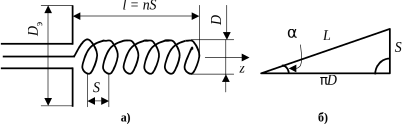
\includegraphics[width=0.8\textwidth]{spyrant.pdf}
	\caption{Цилиндрическая спиральная антенна (а) и развертка ее витка (б)}
	\label{fig:spyrant}
\end{figure}

Экраном может служить металлическая поверхность АР. Выберем оптимальный режим - режим осевого излучения. При этом режиме $L=\lambda$ и угол намотки $\alpha=12^\circ$.

Для углов $\alpha=12\div17^\circ$ применима следующая формула вычисления параметров:

$\displaystyle \Delta\theta_{0.5}=2\theta_\text{ск}=\frac{52^\circ\cdot\lambda}{L}\sqrt{\frac{\lambda}{l}}$

Получаем $\displaystyle l=\frac{52^2\lambda}{4\theta^2_\text{ск}}=\frac{2704\cdot5}{4\cdot324}=10.43 \text{ см}$

Шаг намотки $\displaystyle S=L\cdot sin\alpha=5\cdot sin12^\circ=1.04 \text{ см}$

Диаметр намотки $\displaystyle D=\frac{L\cdot cos\alpha}{\pi}=1.56 \text{ см}$

Количество витков $\displaystyle n=l/S=10.04 \text{ витков}$

Волновое сопротивление излучателя: $\displaystyle Z_\text{вх}=\frac{140\cdot L}{\lambda}=140 \text{ Ом}$


\vfill

{\small \color{gray} Исходные файлы и скрипты для расчёта можно найти в репозитории проекта.}